% Appendix A

\chapter{} % Main appendix title

\label{AppendixA} % For referencing this appendix elsewhere, use \ref{AppendixA}

\lhead{Apéndice} % This is for the header on each page - perhaps a shortened title

Algunas cosas interesantes que faltó incluir en el trabajo. Primero una imagen de algunas versiones de MODI, que fueron posibles por tener acceso a impresoras 3D ya que hacen muy simple el proceso de hacer cambios en los prototipos.

\begin{figure}[htbp]
	\centering
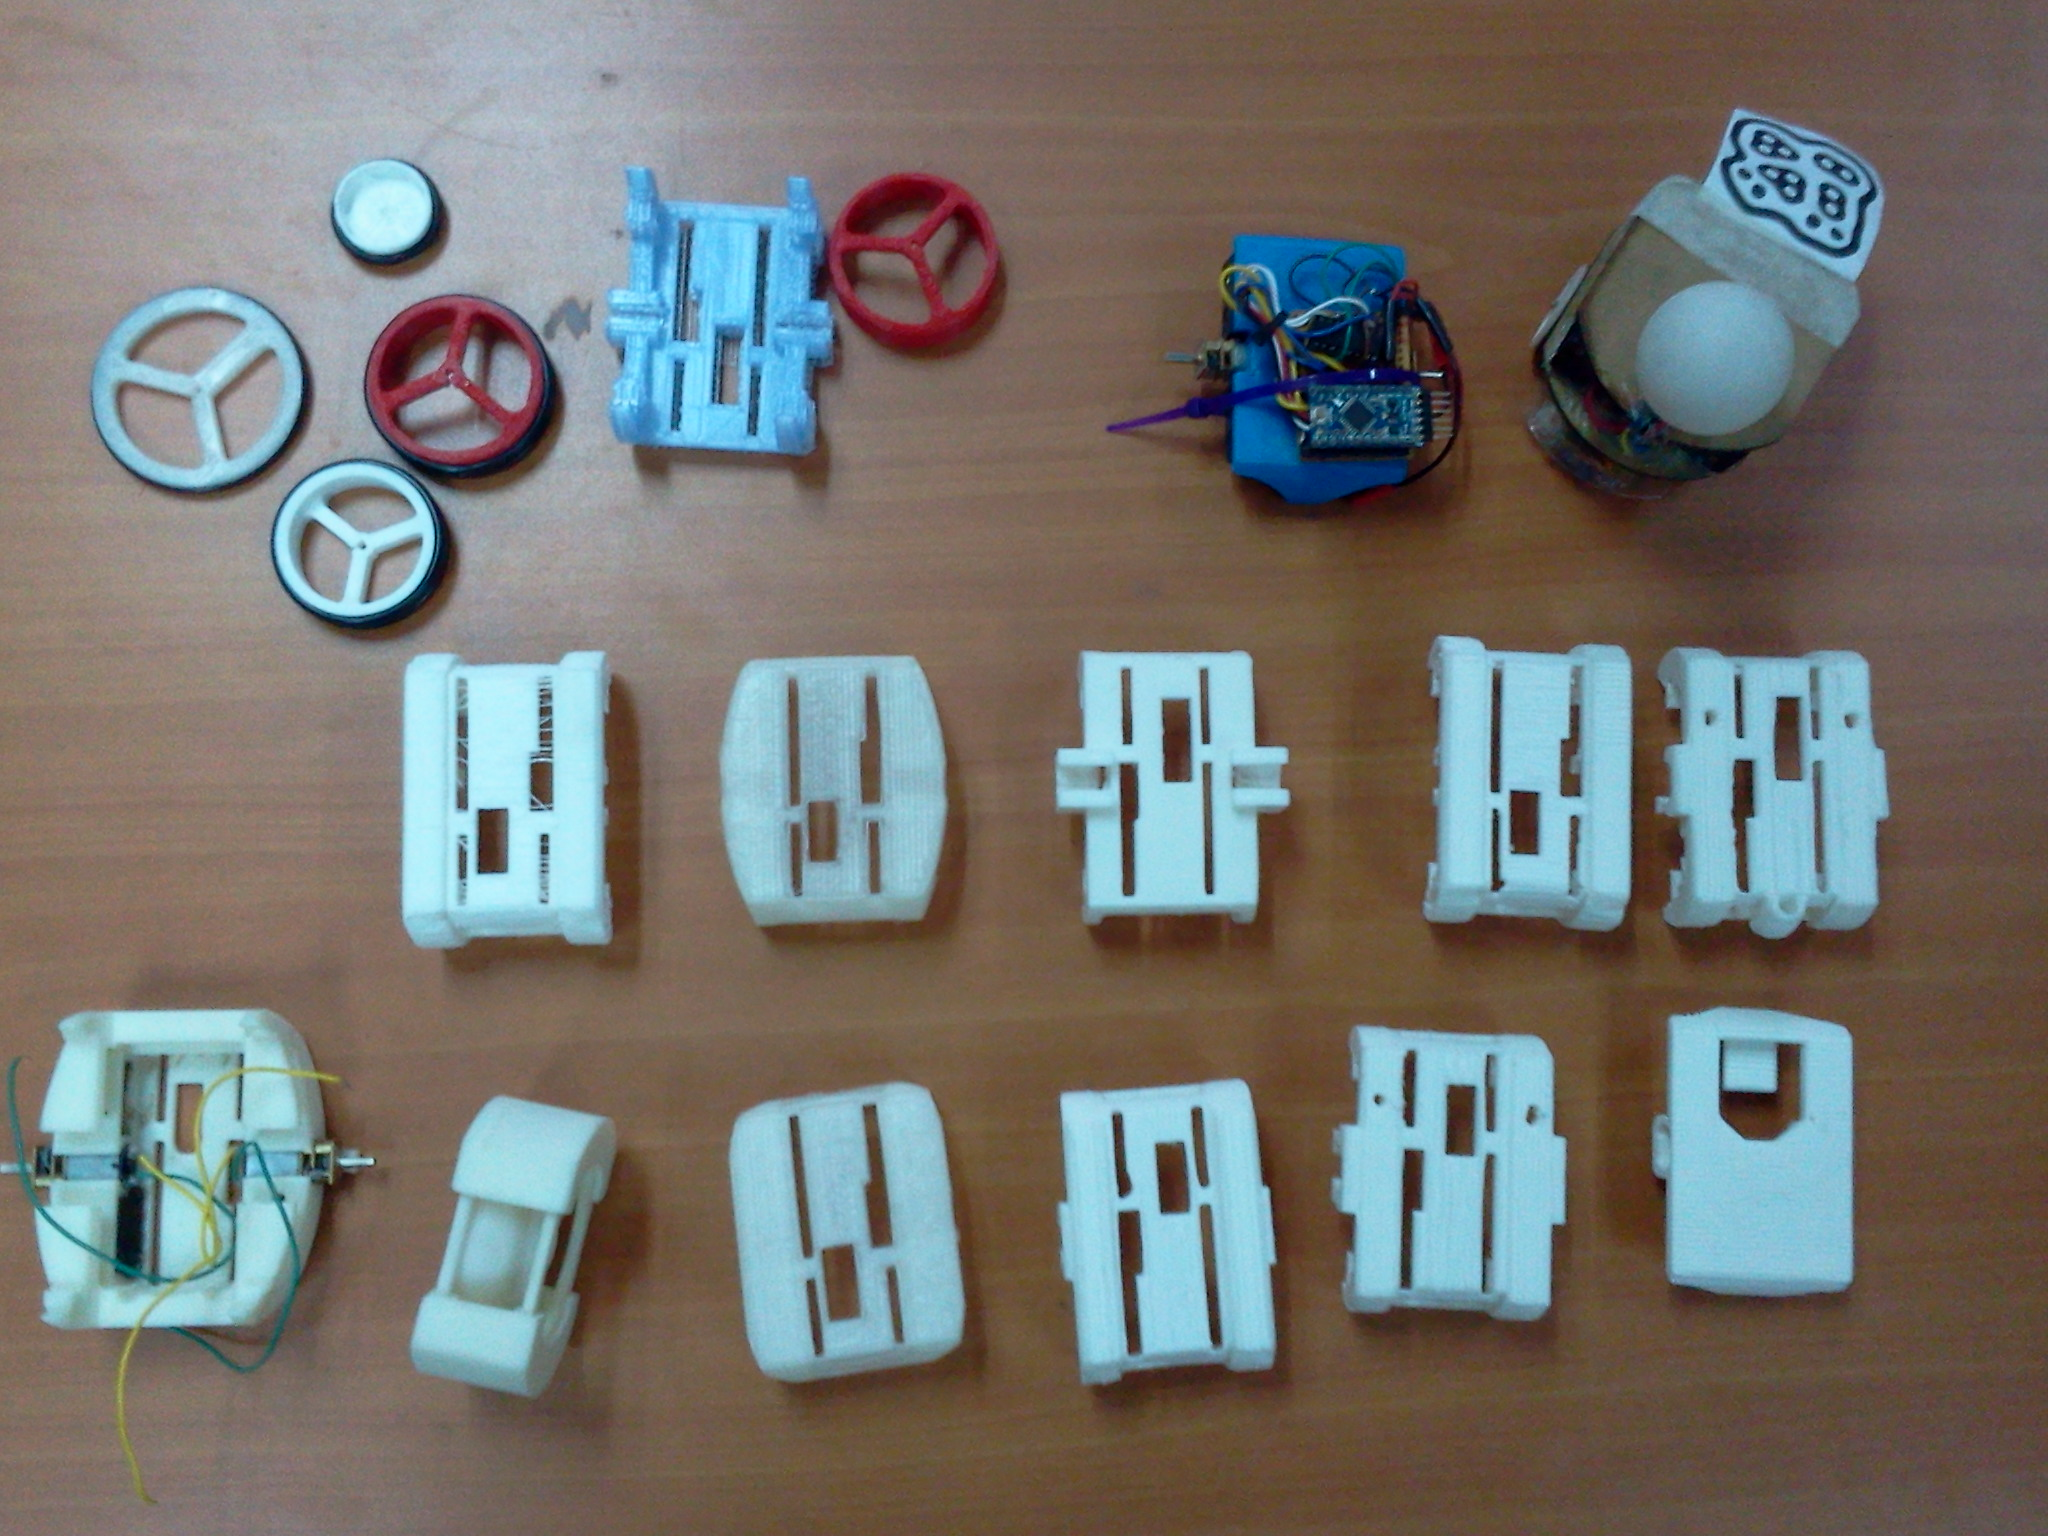
\includegraphics[width=\textwidth]{./Pictures/historia.jpg}
		\rule{35em}{0.5pt}
	\caption[Historia de construcción]{Algunos de los modelos que se construyeron para llegar a la versión final de MODI.}
	\label{fig:Historia}
\end{figure}
Lo segundo es un diagrama con las conexiones eléctricas usadas en el PCB diseñado para MODI.
\begin{figure}[htbp]
	\centering
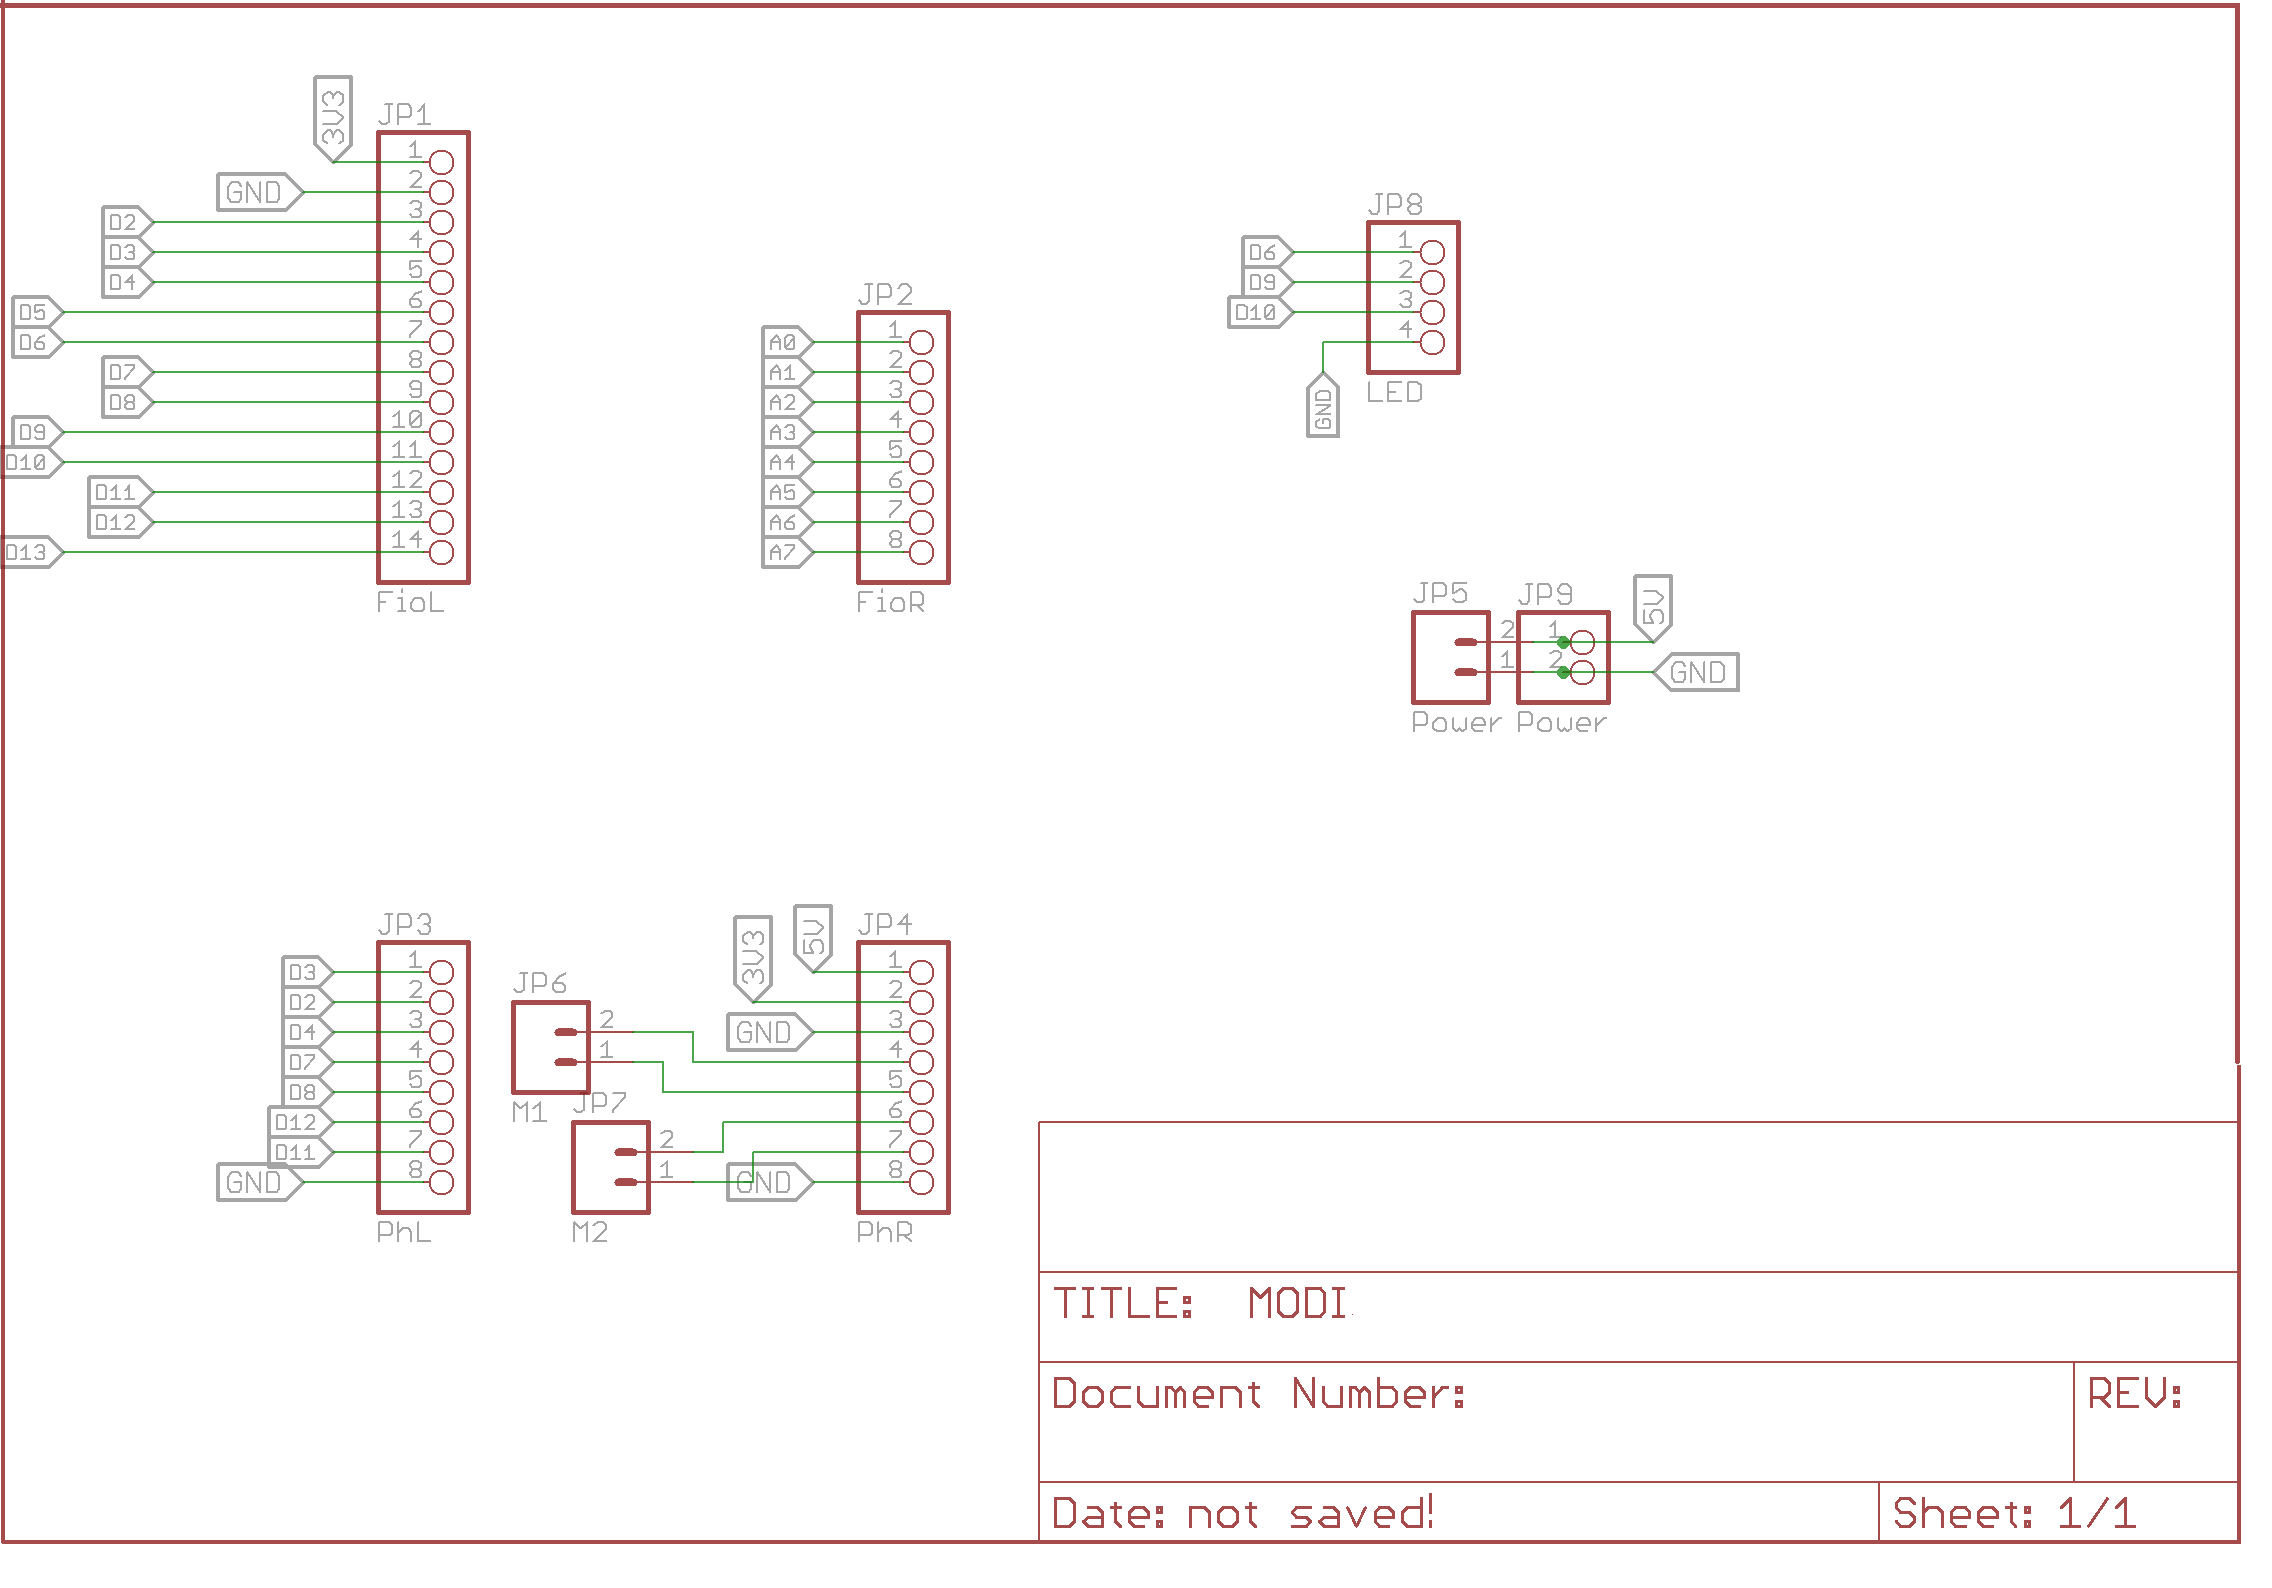
\includegraphics[width=\textwidth]{./Figures/MODI/circuitoPCB.png}
		\rule{35em}{0.5pt}
	\caption[Diagrama eléctrico de conexiones en PCB MODI]{Diagrama de conexiones eléctricas en PCB diseñada para MODI. Está hecho en Eagle 6.4.0.}
	\label{fig:Historia}
\end{figure}
